% \documentclass{article}
\documentclass[12pt,a4paper]{article}
\usepackage{graphicx} % Required for inserting images
\usepackage[a4paper,margin=1in]{geometry}
\usepackage{amsmath, array}
\usepackage[utf8]{inputenc}
\usepackage[T1]{fontenc}
\usepackage{setspace}
\usepackage{graphicx}
\usepackage{titling}
\usepackage{tocloft}
\usepackage{geometry}
\usepackage{amsmath}
\usepackage{ragged2e}
\usepackage{caption}
\usepackage{subcaption}
\usepackage{url}
\usepackage{amsfonts} 
\usepackage{fancyhdr}
\usepackage[utf8]{inputenc}

\usepackage{forest}
\usepackage{xcolor}
\usepackage{amsmath}
\usepackage{amsfonts}
\usepackage{amssymb}
\usepackage{enumitem}
\usepackage{color}
\usepackage{hyperref}
\usepackage{minted}
\usepackage{algpseudocode}

\geometry{left=3cm,right=3cm,top=3cm,bottom=3cm}
\graphicspath{ {images/} }

% --- Header and Footer --- %
\fancypagestyle{plain}{
    \fancyhead{}
    \fancyfoot{}
    \fancyfoot[R]{\thepage}
    \fancyfoot[L]{\textbf{IF2211 - Strategi Algoritma}}
}
\pagestyle{fancy}
\fancyhead{}
\fancyhead[L]{\nouppercase{\rightmark \hfill \leftmark}}
\fancyfoot{}
\fancyfoot[R]{\thepage}
\fancyfoot[L]{\textbf{IF2211 - Strategi Algoritma}}

\renewcommand{\baselinestretch}{1.2} % spacing antar baris

%  Style untuk Daftar Isi
\renewcommand{\contentsname}{Daftar Isi}           % ganti nama contents
\setcounter{tocdepth}{2}                           % tampilkan sampai \subsection

% Judul daftar isi
\renewcommand{\cfttoctitlefont}{\Huge\bfseries}    % font judul TOC
\renewcommand{\cftaftertoctitle}{\par\bigskip}    % jarak setelah judul

% lebar kolom nomor halaman agar rata kanan
\cftsetpnumwidth{2.5em}
\cftsetrmarg{4em}

% Figure prefix
\renewcommand{\figurename}{Gambar}

\begin{document}

\begin{center}
    {\Large \textbf{Laporan Tugas Besar 2}} \\[1.0em]
    {\large \textbf{IF2211 Strategi Algoritma}} \\[0.5em]
    {\large \textsc{Pemanfaatan Algoritma BFS dan DFS dalam Mekanisme Penelusuran CSS pada pohon \textit{Document Object Model}}} \\[0.5em]
    {\normalsize Semester II Tahun 2025/2026} \\[3em]

    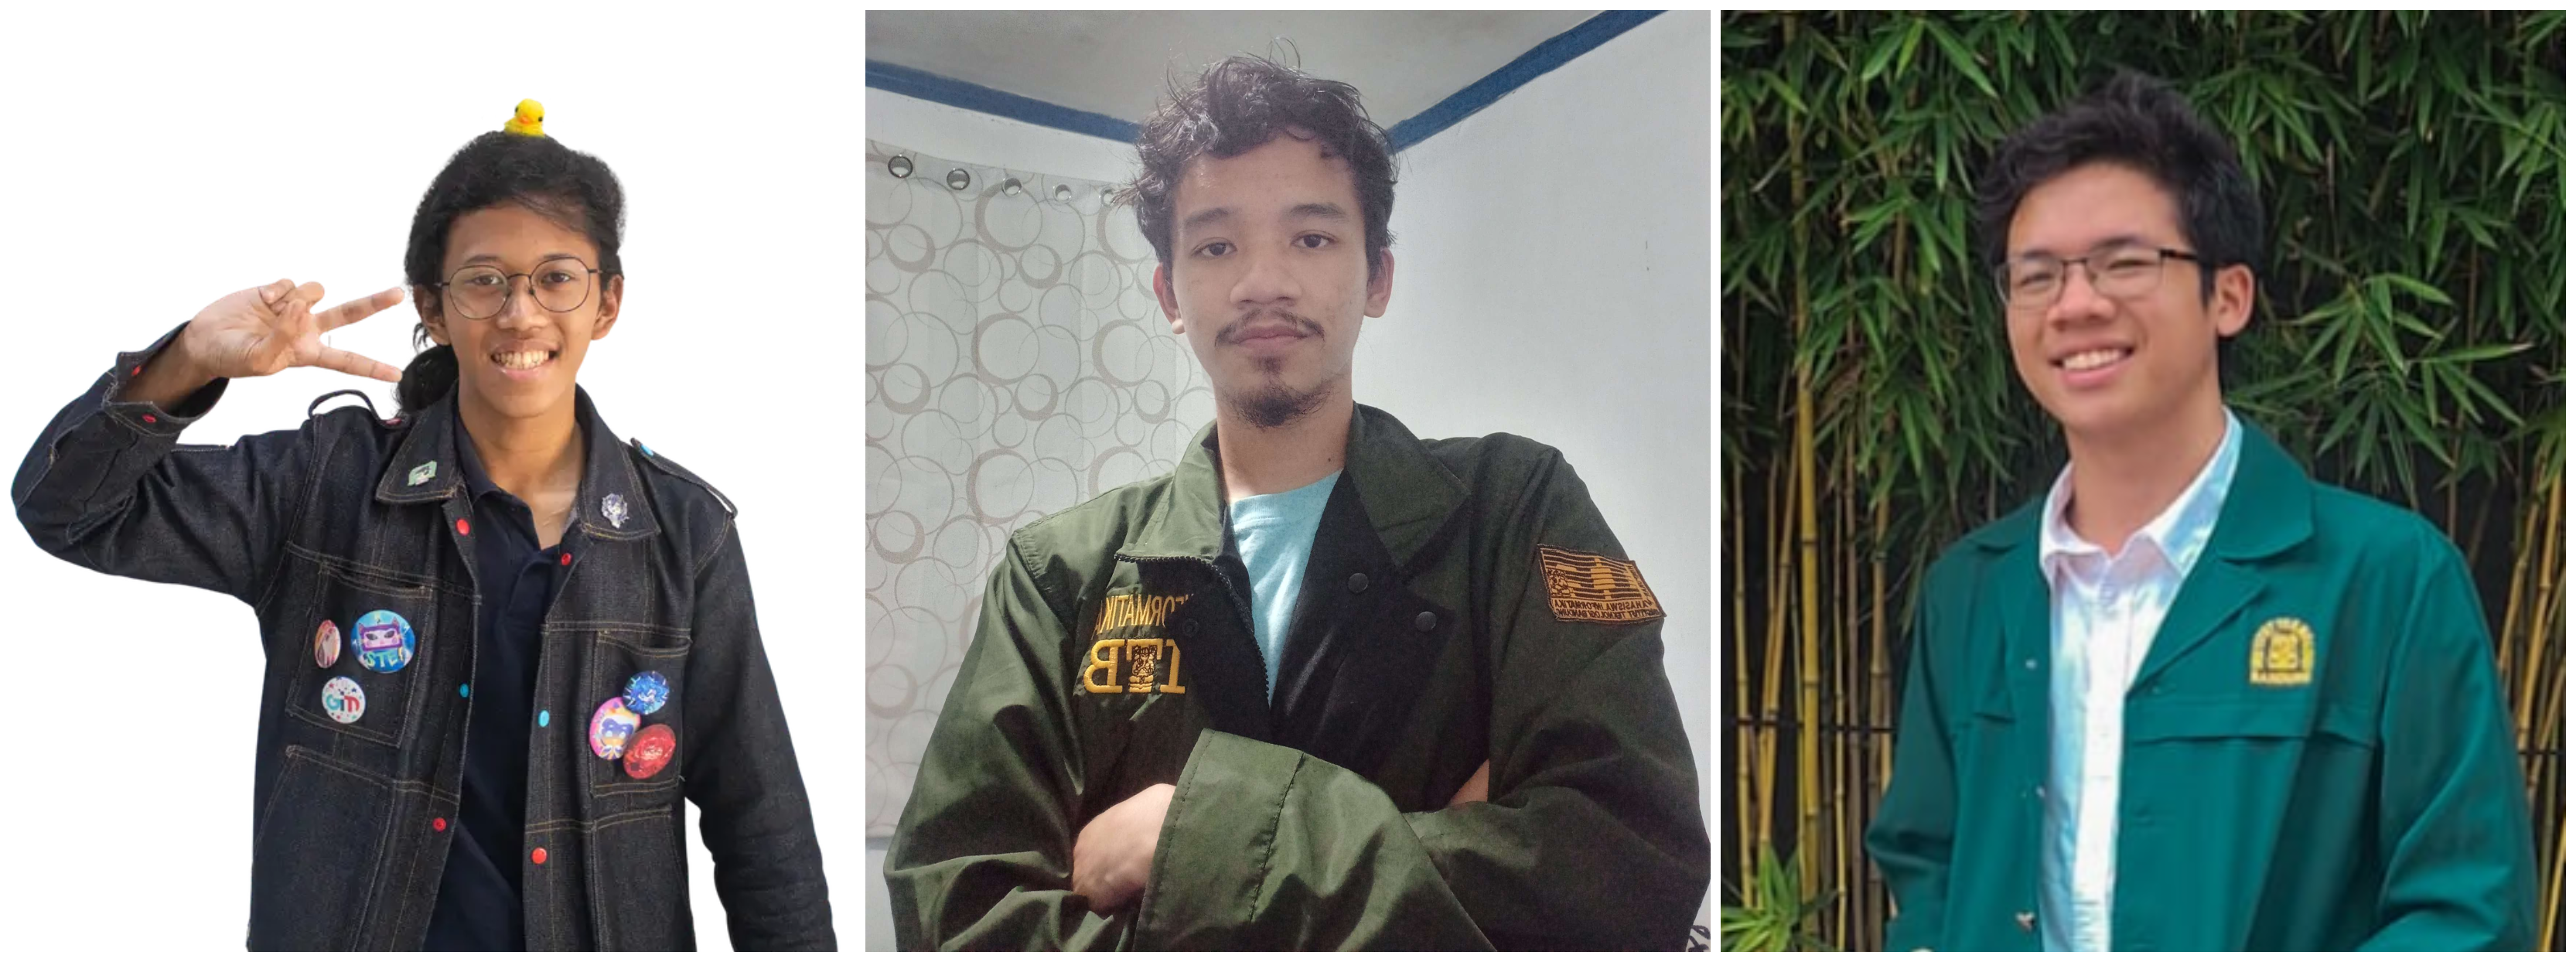
\includegraphics[width=0.45\textwidth]{foto-kelompok.png} \\ [1cm]
    \begin{center}
        \large
        \begin{tabular*}{0.55\textwidth}{@{\hspace{0pt}} l @{\hspace{1cm}} r @{\hspace{0pt}}}
        Muhammad Fatih Irkham Mauludi  & (13524004) \\
        Josh Reinhart Zidik & (13524048) \\
        Jingglang Galih Rinenggan & (13524095) \\
        \end{tabular*}
    \end{center}

    \vfill
    {\large \textsc{Laboratorium Ilmu dan Rekayasa Komputasi}}\\
    {\large \textsc{Program Studi Teknik Informatika}}\\
    {\large \textsc{Sekolah Teknik Elektro dan Informatika}}\\
    {\large \textsc{Institut Teknologi Bandung}}\\
\end{center}

\pagebreak

\tableofcontents

\pagebreak

\section{Deskripsi Tugas}

\begin{figure}[ht]
    \centering
    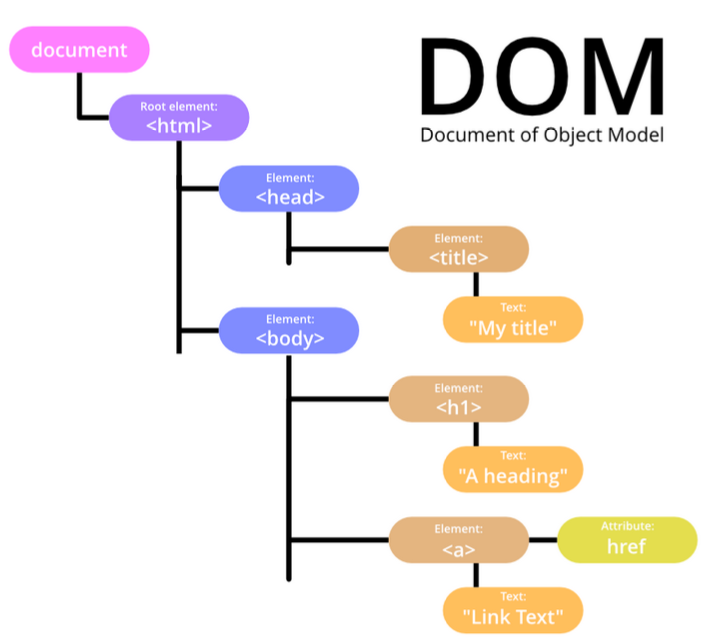
\includegraphics[width=10cm, height=10cm]{section1-dom.png}
    \caption{Struktur Pohon DOM (\textit{Document Object Model})}
    \label{fig:section1-dom}
\end{figure}

Document Object Model (DOM) merupakan representasi terstruktur dari dokumen HTML dalam bentuk tree yang 
memungkinkan setiap elemen pada halaman web diakses, dimodifikasi, dan dimanipulasi oleh program. 
Struktur ini merepresentasikan hubungan antar elemen HTML seperti 
parent, child, dan sibling sehingga memudahkan pengolahan dokumen secara terprogram. \\

Struktur sebuah file HTML pada umumnya meliputi elemen root <html> yang berisi dua bagian utama yaitu <head> dan <body>. 
Bagian <head> berisi metadata seperti judul halaman, link stylesheet, dan script, sedangkan <body> berisi konten utama halaman 
seperti teks, gambar, tombol, dan elemen HTML lainnya yang ditampilkan kepada pengguna. \\

Sebuah website menampilkan sebuah DOM melalui sebuah file bernama Cascading Style Sheets (CSS) yang bertujuan mendeklarasikan visualisasi elemen-elemen pada pohon. 
Deklarasi visualisasi ditempelkan pada elemen-elemen yang berkaitan melalui CSS Selector. \\

Pada Tugas Besar 2 Strategi Algoritma ini, mahasiswa diminta untuk menelusuri dan mencari elemen pada struktur DOM berdasarkan CSS Selector tertentu dengan menggunakan algoritma penelusuran graf yaitu Breadth First Search (BFS) dan Depth First Search (DFS). 
Algoritma tersebut digunakan untuk menjelajahi struktur pohon DOM guna menemukan elemen yang sesuai dengan selector yang diberikan. \\

Komponen-komponen penting yang terdapat pada tugas besar ini antara lain:
\begin{enumerate}
    \item HTML Tags
    \item CSS Selector
    \item HTML parsing
\end{enumerate} \\

Pada tugas ini, terdapat spesifikasi wajib untuk membuat aplikasi traversal pohon HTML (DOM Tree) yang menggunakan algoritma Breadth First Search (BFS) dan Depth First Search (DFS) untuk melakukan pencarian elemen berdasarkan CSS selector pada struktur DOM dengan detail sebagai berikut,
\begin{itemize}
    \item Buatlah sebuah aplikasi berbasis web yang terdiri dari frontend bebas dan backend dalam bahasa \textbf{Go}, \textbf{C#}, \textbf{Rust}, atau \textbf{Typescript} yang mengimplementasikan algoritma \textbf{BFS} dan \textbf{DFS} untuk melakukan penelusuran CSS pada pohon DOM.
    \item Aplikasi dapat melakukan scraping HTML dari sebuah website melalui URL yang diberikan oleh pengguna
    \item Secara umum, berikut adalah input yang diharapkan,
    \begin{enumerate}
        \item URL website atau memasuki teks HTML sendiri
        \item Pilihan algoritma traversal (BFS / DFS)
        \item CSS selector
        \item Jumlah hasil yang ingin ditampilkan:
        \item Top n kemunculan
        \item Semua kemunculan
    \end{enumerate}
    \item HTML yang diperoleh kemudian diparsing menjadi struktur data pohon (DOM Tree).
    \item Output yang diharapkan adalah sebagai berikut:
    \begin{enumerate}
        \item Aplikasi dapat menampilkan visualisasi struktur pohon DOM, disertai dengan keterangan kedalaman maksimum tree
        \item Aplikasi dapat menampilkan highlight pada jalur yang di-traversal oleh algoritma penelusuran yang dipilih untuk menandakan elemen-elemen yang terpengaruh.
        \item Aplikasi dapat menampilkan waktu pencarian serta banyak node yang dikunjungi. 
        \item Setelah melakukan penelusuran, aplikasi menyimpan sebuah traversal log yang memiliki informasi tahapan penelusuran yang dilakukan. 
    \end{enumerate}
\end{itemize} \\

Selain itu terdapat spesifikasi bonus tugas besar (opsional) dengan poin tambahan tertentu yang dapat dipilih dengan detail sebagai berikut,
\begin{itemize}
    \item (4 poin) [Video] Membuat video tentang aplikasi BFS dan DFS pada penelusuran pohon DOM kemudian mengunggahnya di Youtube. Video dibuat harus memiliki audio dan menampilkan wajah dari setiap anggota kelompok.
    \item (5 poin) [Deploy] Aplikasi web yang telah dibuat perlu di deploy menggunakan Microsoft Azure Virtual Machine (VM).
    \item (2 Poin) [Docker] Aplikasi dijalankan menggunakan Docker baik untuk frontend maupun backend.
    \item (6 Poin) [Animasi] Menampilkan animasi penelusuran pohon DOM untuk segala pencarian.
    \item (3 Poin) [Multithreading] Mengimplementasikan multithreading pada algoritma BFS dan/atau DFS untuk melakukan traversal pohon DOM secara paralel. Proses traversal dibagi ke beberapa thread/worker sehingga beberapa node dapat diproses secara bersamaan.
    \item (3 Poin) [LCA Binary Lifting] Mengimplementasikan algoritma Lowest Common Ancestor (LCA) dengan teknik Binary Lifting pada pohon DOM yang dihasilkan.
\end{itemize}

\pagebreak

\section{Landasan Teori}

\pagebreak

\section{Aplikasi DFS dan BFS}


\pagebreak

\section{Implementasi dan Pengujian}

\subsection{Implementasi}

\subsection{Pengujian}

\pagebreak


\section{Kesimpulan dan Saran}

\subsection{Kesimpulan}

\subsection{Saran}

\pagebreak

\section*{Daftar Pustaka}

\renewcommand{\refname}{}
\vspace{-2em}

\begin{thebibliography}{}

\bibitem{munir-graph-1}
Rinaldi Munir (2026), \texit{Breadth/Depth First Search (BFS/DFS) (Bagian 1)}, https://informatika.stei.itb.ac.id/~rinaldi.munir/Stmik/2025-2026/13-BFS-DFS-(2026)-Bagian1.pdf

\bibitem{munir-graph-2}
Rinaldi Munir (2026), \texit{Breadth/Depth First Search (BFS/DFS) (Bagian 2)}, https://informatika.stei.itb.ac.id/~rinaldi.munir/Stmik/2025-2026/14-BFS-DFS-(2026)-Bagian2.pdf

\end{thebibliography}

\pagebreak


\section*{Pernyataan Orisinilitas}
Tugas ini disusun sepenuhnya tanpa bantuan kecerdasan buatan (\textit{Generative AI}), melainkan hasil pemikiran dan analisis mandiri.

\begin{flushright}
    \vspace{0.5cm}
    
\includegraphics[width=3cm]{ttd-fatih.png} \\
    \rule{5cm}{0.4pt} \\
    \vspace{0.5cm}
    Muhammad Fatih Irkham Mauludi (13524004)
\end{flushright}

\begin{flushright}
    \vspace{0.5cm}
    
\includegraphics[width=3cm]{ttd-josh.png} \\
    \rule{5cm}{0.4pt} \\
    \vspace{0.5cm}
    Josh Reinhart Zidik (13524048)
\end{flushright}

\begin{flushright}
    \vspace{0.5cm}
    
\includegraphics[width=3cm]{ttd-cikang.png} \\
    \rule{5cm}{0.4pt} \\
    \vspace{0.5cm}
    Jingglang Galih Rinenggan (13524095)
\end{flushright}

\pagebreak

\section*{Lampiran}

\begin{itemize}

\item Repository Github: \\ \url{https://github.com/FieryBanana101/Tubes2_kata-josh-nama-timnya-jangan-ini} 

\end{itemize}

\begin{table}[h]
    \centering
    \caption{Checklist hasil}
    \begin{tabular}{|c|p{12cm}|c|c|}
        \hline
        \textbf{No} & \textbf{Poin} & \textbf{Ya} & \textbf{Tidak} \\
        \hline
        1. & Aplikasi berhasil di kompilasi tanpa kesalahan & & &
        \hline
        2. & Aplikasi berhasil dijalankan &  & &
        \hline
        3. & Aplikasi dapat menerima input URL web, pilihan algoritma, CSS selector, dan jumlah hasil & & &
        \hline
        4. & Aplikasi dapat melakukan scraping terhadap web pada input  & & &
        \hline
        5. & Aplikasi dapat menampilkan visualisasi pohon DOM & & & 
        \hline
        6. & Aplikasi dapat menelusuri pohon DOM dan menampilkan hasil penelusuran & & & 
        \hline
        7. & Aplikasi dapat menandai jalur tempuh oleh algoritma  &  & &
        \hline
        8. & Aplikasi dapat menyimpan jalur yang ditempuh algoritma dalam traversal log  &  & &
        \hline
        9. & [Bonus] Membuat video  &  & &
        \hline
        10. & [Bonus] Deploy aplikasi  &  & &
        \hline
        11. & [Bonus] Implementasi animasi pada penelusuran pohon  &  & &
        \hline
        12. & [Bonus] Implementasi multithreading  &  & &
        \hline
        13. &  [Bonus] Implementasi LCA Binary Lifting &  & &
        \hline
    \end{tabular}
\end{table}


\begin{table}[h]
    \centering
    \caption{Pembagian Tugas Kelompok}
    \begin{tabular}{|c|p{5cm}|c|c|}
        \hline
        \textbf{No} & \textbf{Anggota} & \textbf{Detail Tugas} & \textbf{Presentase Keseluruhan} \\
        \hline
        1. & Muhammad Fatih Irkham Mauludi (13524004) & & &
        \hline
        2. & Josh Reinhart Zidik (13524048) & & &
        \hline
        3. & Jingglang Galih Rinenggan (13524095) & & &
        \hline
    \end{tabular}
\end{table}















\pagebreak

\end{document}
